\section{Żadanie adresacji}
Tutaj po raz pierwszy można zaobserwować zmienioną wartość pola adresu dla wiadomości
przychodzącej. Oznacza to, że urządzenie podrzędne zaakceptowało żadanie adresacji 
oraz identyfikuje się w trakcie rozmowy z urządzeniem nadrzędnym pod adresem 0x03 co
jest prawdą dla każdej następnej wiadomości.

Analiza wartości wiadomości wychodzącej 
(rysunek \ref{lst:WykonanieProgramu}, linijki {20, 21} oraz \ref{fig:DiagramSequence_AddressAssignment_SecondDeviceScan}):
\begin{enumerate}
    \item ADDR = 0xFF --- broadcast;
    \item CTRL = 0xBF --- charakterystyczny dla ramki XID;
    \item FI = 0x81 --- charakterystyczna dla ramki XID oraz grupy wiadomości przypisania adresu;
    \item GI = 0xF0 --- grupa wiadomości przypisania adresu;
    \item GL = 0x11;
    \item Pierwszy parametr HDLC:
    \begin{enumerate}
        \item PI = 0x01 --- unikalny identyfikator urządzenia podrzędnego;
        \item PL = 0x09;
        \item PV = \{ 0x4E, 0x4B, 0x34, 0x36, 0x35, 0x30, 0x30, 0x30, 0x30 \};
    \end{enumerate}
    \item Drugi parametr HDLC:
    \begin{enumerate}
        \item PI = 0x02 --- docelowy adres urządzenia podrzędnego;
        \item PL = 0x01;
        \item PV = 0x03;
    \end{enumerate}
    \item Trzeci parametr HDLC:
    \begin{enumerate}
        \item PI = 0x04 --- typ urządzenia podrzędnego;
        \item PL = 0x01;
        \item PV = 0x01 --- pojedynczy RET;
    \end{enumerate}
\end{enumerate}

\begin{figure}[h!]
    \centering
    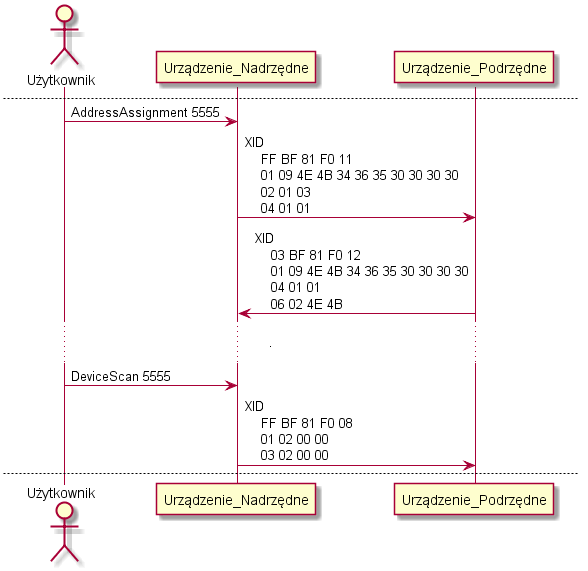
\includegraphics[scale=0.75]{out/Diagramy/UML_DiagramOfSequence_New/UML_DiagramOfSequence_New-page2.png}
    \caption{Żadanie adresacji oraz dodatkowe skanowanie urządzeń.
        \newline(Opracowanie własne)}
    \label{fig:DiagramSequence_AddressAssignment_SecondDeviceScan}
\end{figure}
